\documentclass{astroedu-lab}

\begin{document}

\pagestyle{plain}

\begin{problem}{\huge Лабораторная работа 2.1.4\\\\Определение теплоемкости\\\\твердых тел\\\\Выполнил Жданов Елисей Б01-205}

\section{Цель работы:}

1) Прямое измерение кривых нагревания и охлаждения пустого калориметра и системы «калориметр + твердое тело»
 
2) Определение коэффициента теплоотдачи стенок калориметра

3) Определение теплоемкости пустого калориметра и удельной теплоемкости твердого тела

\section{Оборудование:}

Калориметр с нагревателем и термометром сопротивления

Вольтметр в режиме омметра, измеритель температуры

Источник питания, амперметр и вольтметр для измерения мощности нагревателя

Компьютерная программа АКИП

\section{Теоретическая справка}

Существует несколько способов расчета параметров данной термодинамической системы

Рассмотрю сначала интергральный метод. Он заключается в получении зависимости T(t) путем интегрирования дифференциального уравнения теплообмена

\begin{equation}
	C dT_{cool} = -\lambda [T_{cool} - T_k] dt
\end{equation}

Откуда

\begin{equation}
	\boxed{ln \frac{T_{cool} - T_k}{T - T_k} = \frac{-\lambda}{C} t}
\end{equation}

Это уравнение имеет линейный вид в логарифмических координатах, из которых с легкостью находится $\frac{\lambda}{C}$

Записав похожее уравнение для нагрева, получу

\begin{equation}
	\boxed{T_{heat}(t) = \frac{P}{\lambda} \left(1 - e^{\frac{-\lambda}{C}t}\right) + T_k}
\end{equation}

По коэффициентам для соответствующих уравнений прямых $\frac{\lambda}{C}$ и $\frac{P}{\lambda}$ находятся $\lambda$ и С.

Интегральный метод дает хорошие результаты только при небольших колебаниях комнатной температуры, в противном случае более оправданным будет дифференциальные методы

Один из них заключается в рассмотрении удобной точки при $T = T_{\text{комн}}$.

\begin{equation}
	\boxed{C = \frac{P}{(dT/dt)_{T = T_\text{комн}}}}
\end{equation}

Другой метод заключается в нахождении производной в 2-х точках нагрева-охлаждения с одинаковой температурой. Тогда

\begin{equation}
	\boxed{\lambda = \frac{P}{(T - T_{k2})\left( 1 - \frac{A}{B} \right) + T_{k2} - T_{k1}}}
\end{equation}

\begin{equation}
	\boxed{C = \frac{P}{A - B + A \frac{T_{k1} - T_{k2}}{T-T_{k1}}}}
\end{equation}

Где $A = \left(\frac{dT}{dt}\right)_{heat}$ и $B =\left( \frac{dT}{dt}\right)_{cool}$

 
\section{Экспериментальная установка}

Система реостатов на рисунке позволяет установить нужную силу тока в цепи нагревателя. По амперметру и вольтметру определяется мощность, выделяемая в нагревателе. Величина сопротивления термометра измеряется мостом постоянного тока.

\begin{figure}[!h]
	\centering
	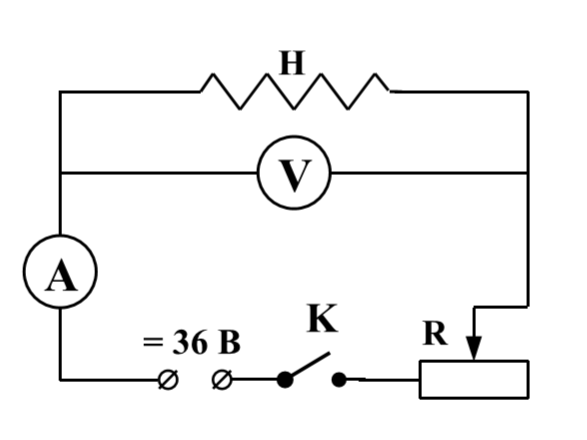
\includegraphics[width=0.4\textwidth]{Схема нагревателя.png}
	\label{fig:boiler}
\end{figure}

\section{Измерения}

Зафиксирую напряжение и ток, подаваемые на нагреватель

U = 27.26 Вольт

I = 0.2268 Ампер

\begin{equation}
	P = UI = (6.182 \pm 0.005) \text{Вт}
\end{equation}

Запишу массы всех конусов для расчета удельный теплоемкости

\begin{center}
\begin{tabular}{|c|c|}
\hline
& m, гр \\
\hline
Латунь & $(875.5 \pm 0.1)$ \\
Железо & $(815.1 \pm 0.1)$ \\
Алюминий & $(294.2 \pm 0.1)$ \\
\hline
\end{tabular}
\end{center}

Проверю, что подаваемая мощность не будет меняться с течением эксперимента

Подготовлю ПО и включу замеры.

Буду протирать латунный конус тчательно, чтобы избежать попадания водяного пара в установку и, как слудствие, изменения итоговой теплоемкости.

В результате успел провести два замера на нагрев и охлаждение пустого калориметра, один замер алюминиевого конуса и замер на нагрев железного конуса.

\subsection{Журнал наблюдений}

    14:32 - конус из латуни холодный положили
	
	14:38 - конус из латуни вынули
	
	14:44 - включили GPS-72
	
	15:13 - выключили GPS-72
	
	15:20 - конус из латуни холодный положили
	
	15:23 - температура начала расти
	
	15:26 - конус из латуни вынули
	
	15:29 - включили GPS-72

	15:47 - выключили GPS-72

	15:54 - конус из латуни холодный положили

	15:57 - температура начала расти

	16:00 - конус из латуни вынули и вставили алюминиевый конус

	16:05 - включили GPS-72

	16:24 - выключили GPS-72

	16:35 - конус из алюминия вынули и вставили латунь холодный конус

	16:38 - вынули латунь и вставили железный конус

	16:41 - включили GPS-72

\section{Обработка}

Загружу полученные файлы на пк и приступлю к обработке

Обрежу лишние данные и преобразую измерения в требуемый вид.

Для используемой 1 установки формула преобразования сопротивления в температуру

\begin{equation}
	T(R_T)= 14.37798 \cdot R_T + 39.35514
\end{equation}

Построю суммарный график для определения необходимых временных интервалов

\begin{center}
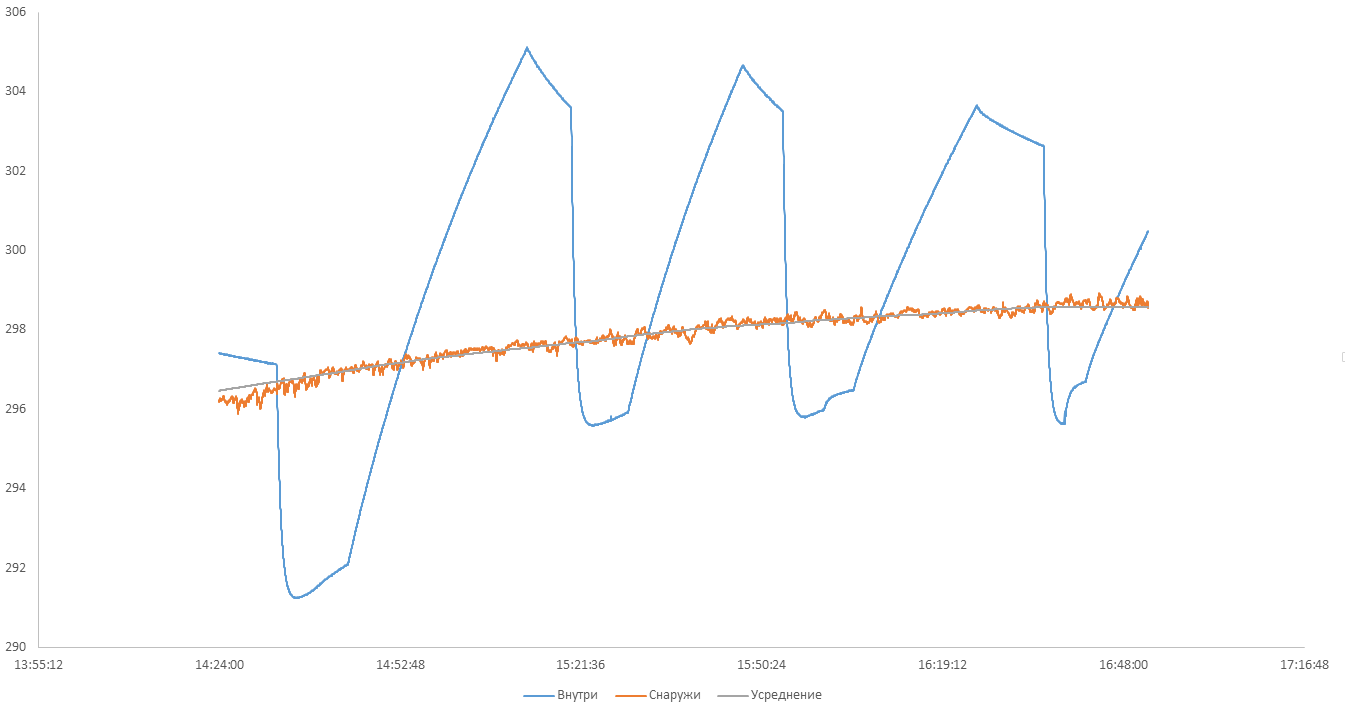
\includegraphics[width=1\textwidth]{total.png}
\label{ris:image}
\end{center}

Добавлю усреднение скользящей средней по 1000 значениям для комнатной температуры. Как видно, оно довольно хорошо описывает среднюю температуру в любой момент времени.

\subsection{Интегральный метод}

Рассмотрю промежутки охлаждения

\begin{center}
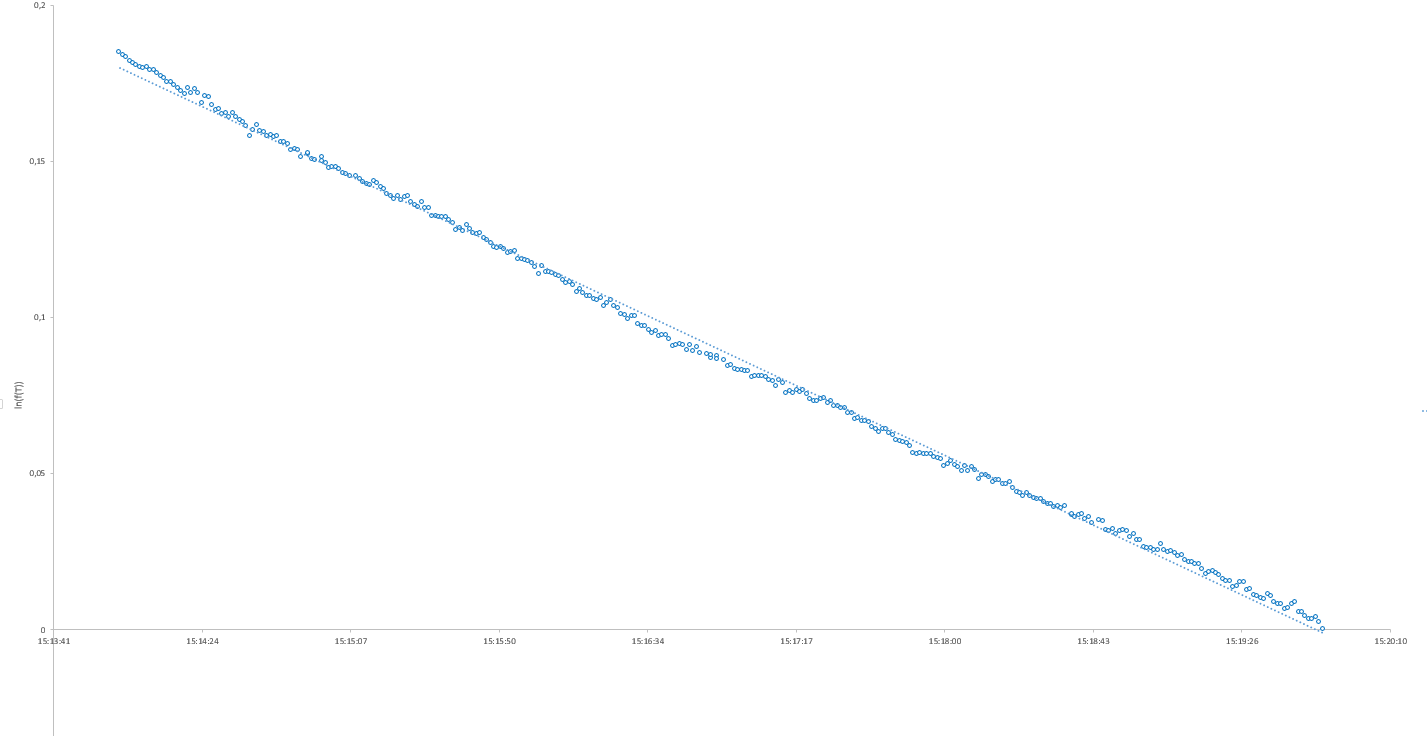
\includegraphics[width=1\textwidth]{картинки/2023-02-10_01-26-06.png}
\label{ris:image}
\end{center}

Охлаждение пустого калориметра 1

\begin{center}
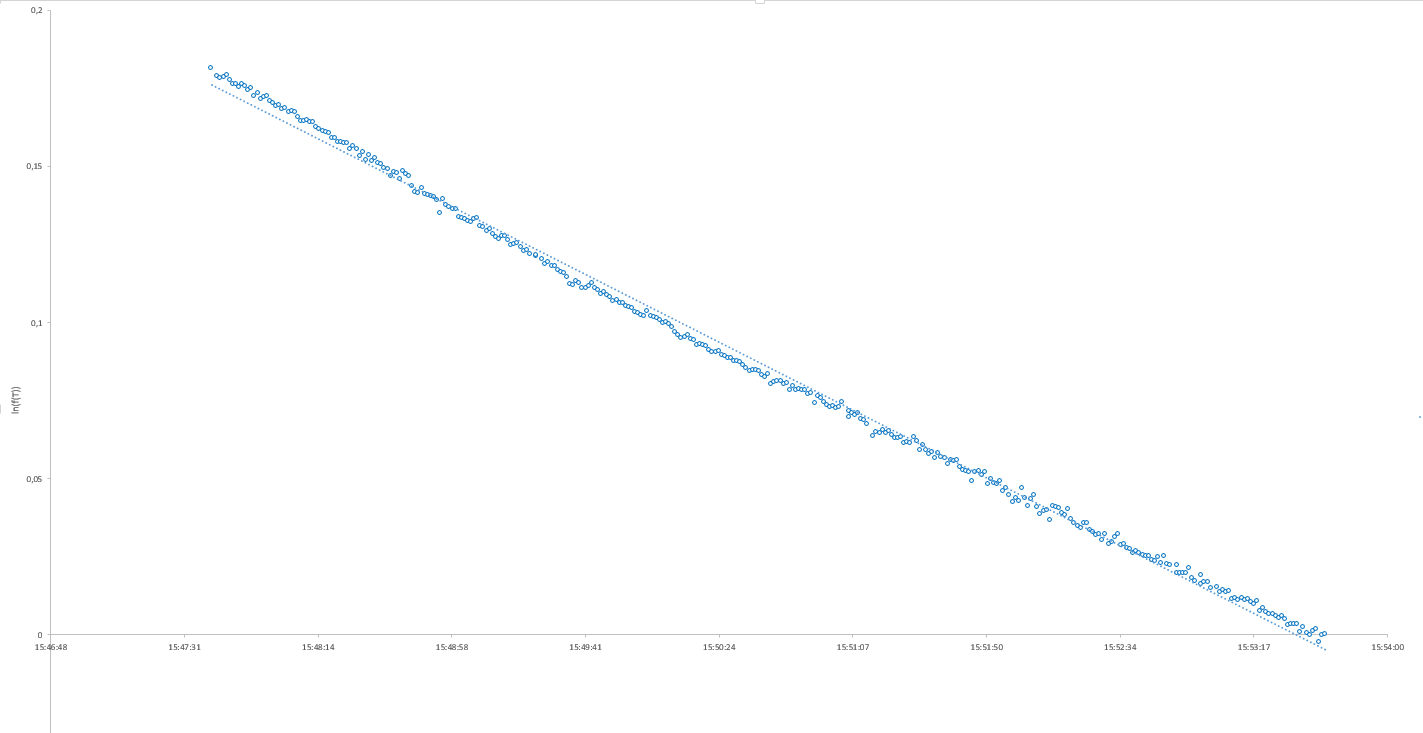
\includegraphics[width=1\textwidth]{картинки/2023-02-10_01-46-44.png}
\label{ris:image}
\end{center}

Охлаждение пустого калориметра 2

\begin{center}
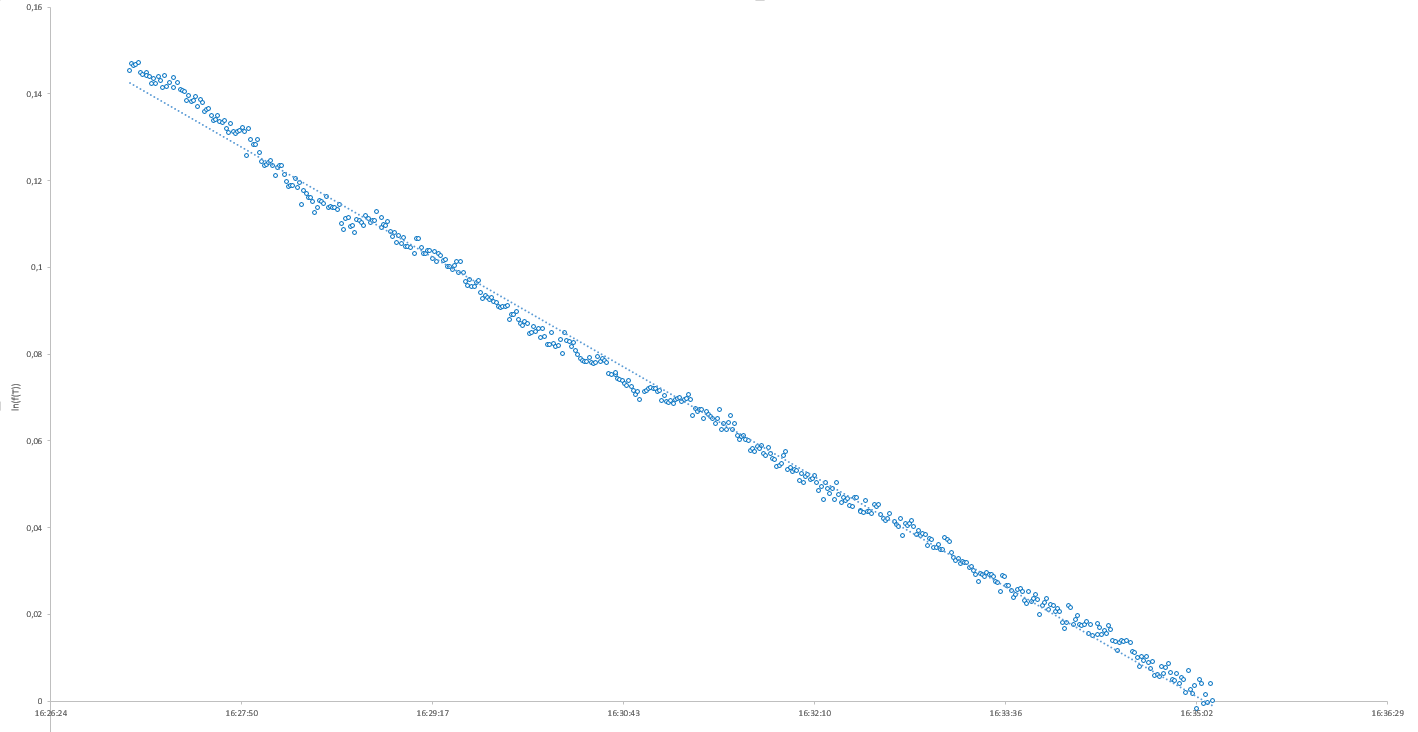
\includegraphics[width=1\textwidth]{картинки/2023-02-10_01-54-50.png}
\label{ris:image}
\end{center}

Охлаждение калориметра с алюминием

Как видно, начальный момент достаточно отделен от момента отключения нагрева, поскольку отклонение от аппроксимирующей прямой при меньшем времени укладывается в пределы разброса остальных точек

Найду угловые коэффициенты прямых для каждой установки по МНК.

\[
	a = \frac{n \sum_{i=1}^n N_i \nu_i - \left( \sum_{i=1}^n N_i \right) \left( \sum_{i=1}^n \nu_i \right)}{n \sum_{i=1}^n N_i^2 - \left( \sum_{i=1}^n N_i \right)^2}
\]

\[
	b = \frac{\sum_{i=1}^n \nu_i - a \sum_{i=1}^n N_i}{n}
\]

Также рассчитаю их погрешности

\begin{equation}
	S_a^2 = \frac{\sum_{i=1}^n N_i^2}{n \sum_{i=1}^n N_i^2 - \left( \sum_{i=1}^n N_i \right)^2} \cdot \frac{\sum_{i=1}^n \left( \nu_i - b - a \cdot N_i \right)^2}{n - 2}
\end{equation}

Результат приведу в таблице ниже

Построю также графики нагрева калориметра от времени.

Начало графиков соответствует моменту времени пересечения графиком температуры внутри калориметра усреднения для комнатной температуры

\begin{center}
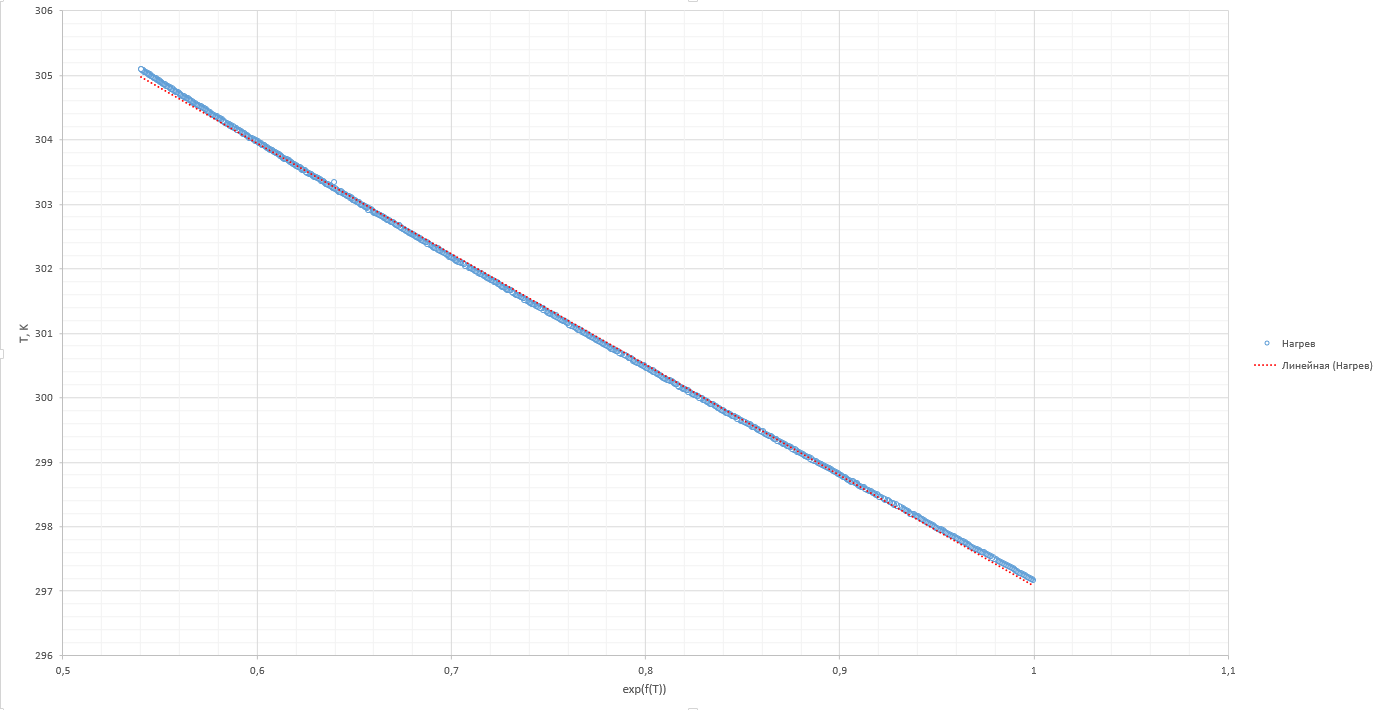
\includegraphics[width=1\textwidth]{картинки/2023-02-11_14-58-31.png}
\label{ris:image}
\end{center}

Нагрев пустого калориметра 1

\begin{center}
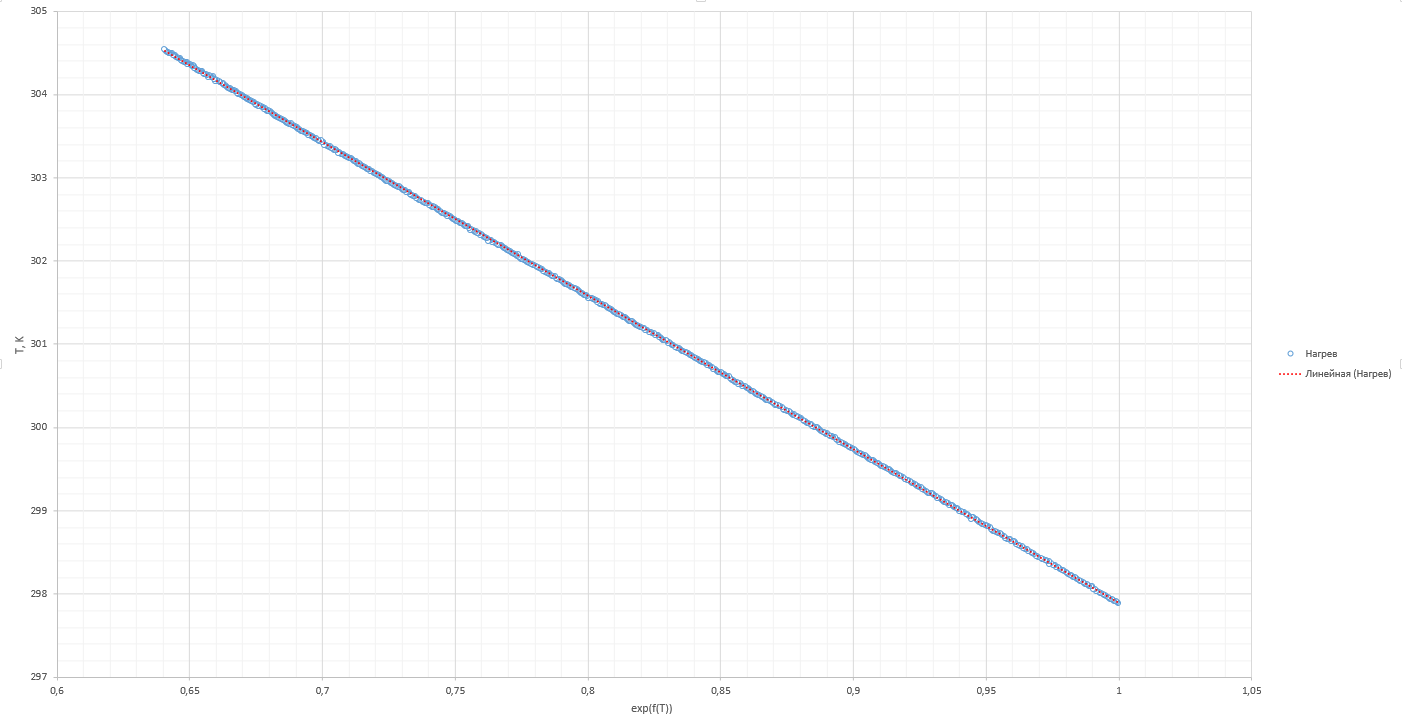
\includegraphics[width=1\textwidth]{картинки/2023-02-11_14-57-54.png}
\label{ris:image}
\end{center}

Нагрев пустого калориметра 2

\begin{center}
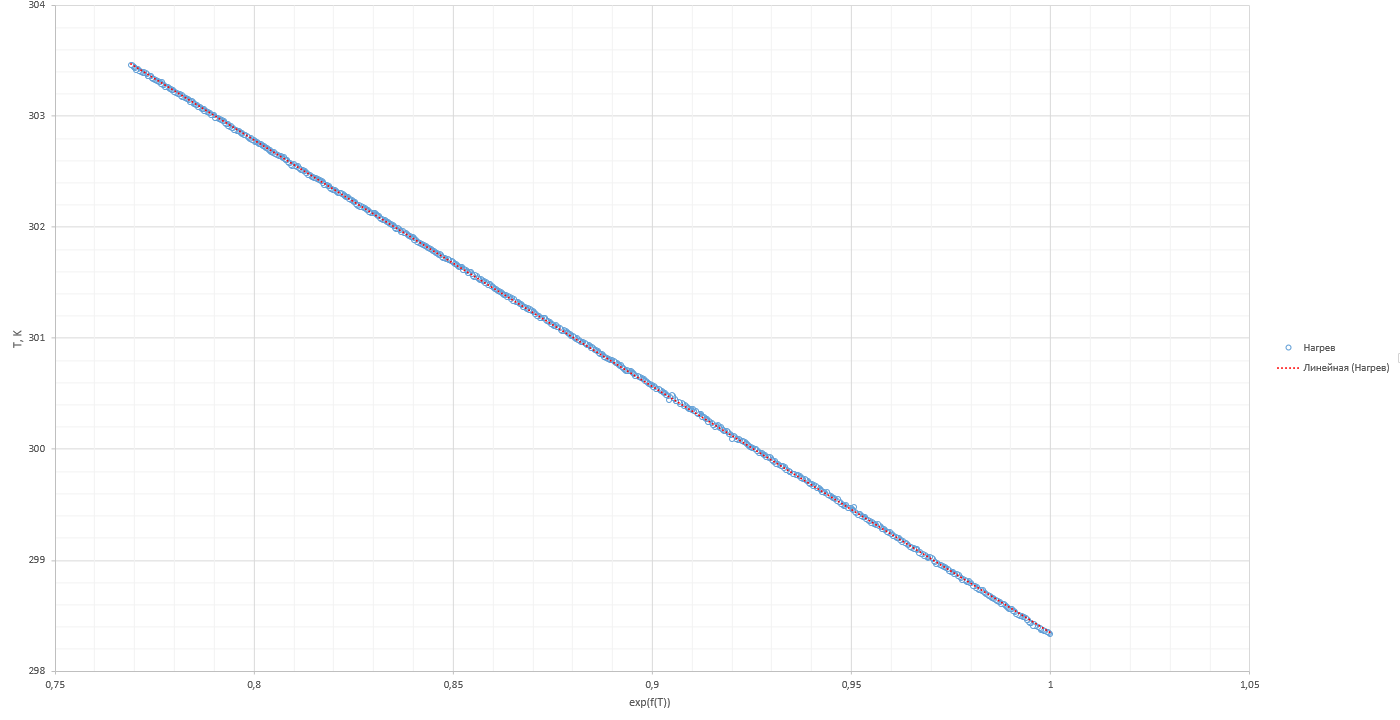
\includegraphics[width=1\textwidth]{картинки/2023-02-11_14-54-42.png}
\label{ris:image}
\end{center}

Нагрев калориметра с алюминием

Составляю таблицу

\begin{center}
\begin{tabular}{|c|c|c|c|c|}
\hline
 & $\frac{P}{\lambda}$ & $\frac{\lambda}{C}$ & C, $\frac{\text{Дж}}{K}$ & $\lambda$, $\frac{\text{Вт}}{K}$ \\ \hline
Пустой 1 & $(17.184 \pm 0.015)$ & $(0.0005162 \pm 0.0000012)$ & $(697 \pm 3) $ & $(0.3598 \pm 0.0006)$ \\
Пустой 2 & $(18.432 \pm 0.004)$ & $(0.0005027 \pm 0.0000014)$ & $(667 \pm 3)$ & $(0.3354 \pm 0.0003) $\\
Алюминий & $(22.173 \pm 0.006)$ & $(0.0002932 \pm 0.0000007)$ & $(951 \pm 3)$ & $(0.2788 \pm 0.0003)$\\
\hline
\end{tabular}
\end{center}

Относительные погрешности $\lambda$ и C определяются суммой относительных погрешностей компонент.

\subsection{Дифференциальный метод пересечения комнатной\\ температуры}

Теперь построю графики зависимости T(t) около средней комнатной температуры

\begin{figure}
		\begin{center}
			\begin{minipage}[h]{0.48\linewidth}
				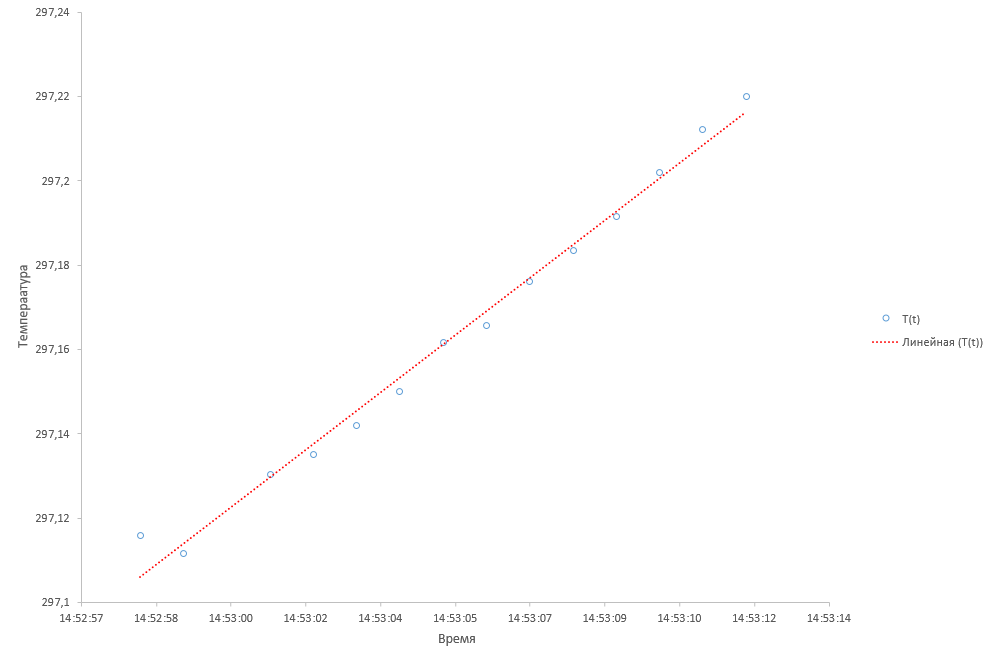
\includegraphics[width=1\linewidth]{картинки/2023-02-11_22-50-46.png}
				\caption{Пустой калориметр 1} %% подпись к рисунку
				\label{ris:dR_dt(r)_for_calorimetr} %% метка рисунка для ссылки на него
			\end{minipage}
		\hfill
			\begin{minipage}[h]{0.48\linewidth}
				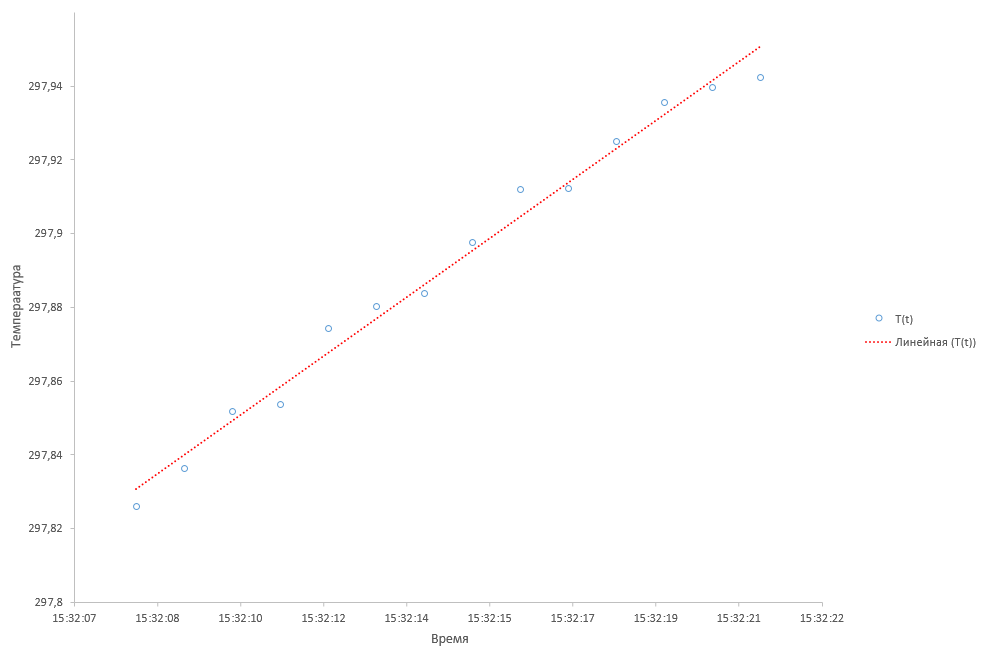
\includegraphics[width=1\linewidth]{картинки/2023-02-11_22-51-37.png}
				\caption{Пустой калориметр 2}
				\label{ris:dR_dt(r)_for_steel}
			\end{minipage}
		\end{center}
		\begin{center}
			\begin{minipage}[h]{0.48\linewidth}
				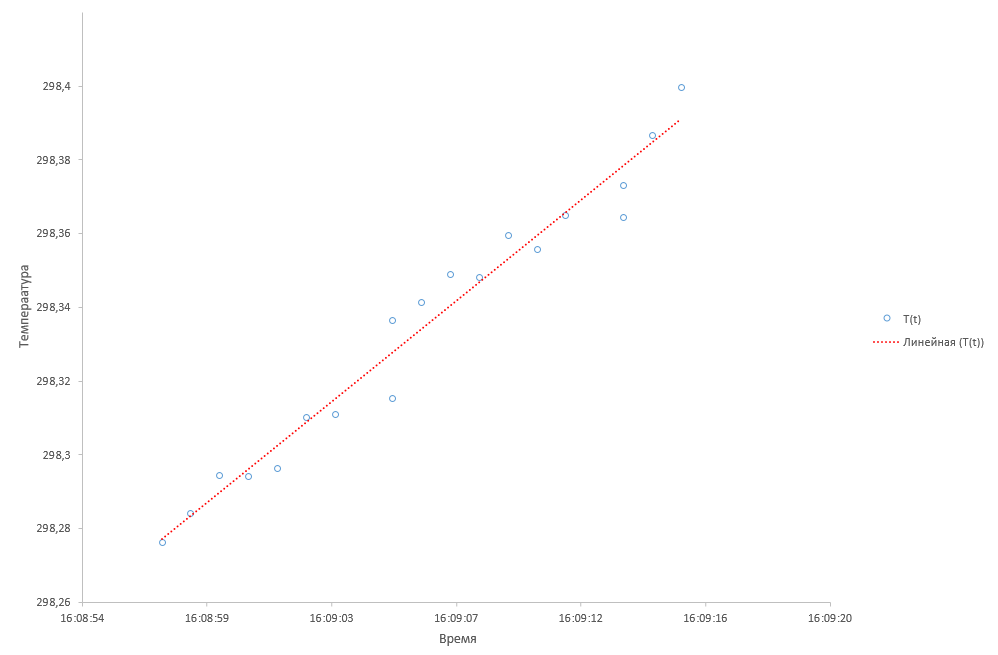
\includegraphics[width=1\linewidth]{картинки/2023-02-11_22-52-18.png}
				\caption{Алюминий} 
				\label{ris:dR_dt(r)_for_latun'} %% метка рисунка для ссылки на него
			\end{minipage}
		\hfill
			\begin{minipage}[h]{0.48\linewidth}
				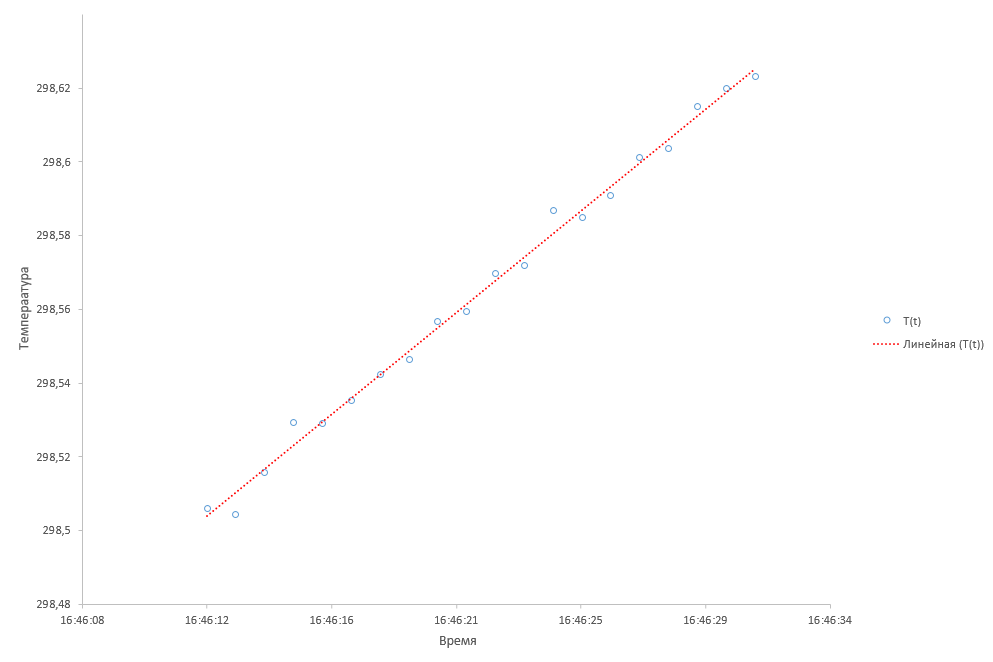
\includegraphics[width=1\linewidth]{картинки/2023-02-11_22-53-10.png}
				\caption{Железо}
				\label{ris:dR_dt(r)_for_aluminium}
			\end{minipage}
		\end{center}
\end{figure}

\newpage

С помощью стандартных формул МНК получу коэффициент наклона графиков, а по нему теплоемкости

\begin{center}
\begin{tabular}{|c|c|c|}
\hline
 & $\frac{P}{C}$ & $C$, $\frac{\text{Дж}}{K}$ \\ \hline
Пустой 1 & $(0.00832 \pm 0.00021)$ & $(740 \pm 20)$ \\
Пустой 2 & $(0.00924 \pm 0.00034)$ & $(670 \pm 30)$ \\
Алюминий & $(0.0064  \pm 0.00023)$ & $(970 \pm 40)$ \\
Железо &   $(0.00638 \pm 0.00012)$&  $(970 \pm 20)$ \\
\hline
\end{tabular}
\end{center}

Как видно, дифференциальный метод сопряжен с неточностями, и даже в первых двух идентичных(с точки зрения проведения) экспериментов дает довольно сильно отличающиеся значения.

Тем не менее, точность метода достаточна для принятия замеров достоверными

\subsection{Дифференциальный метод изотерм}

Приведу сначала графики зависимости T(t) для температур, близких к 304 K у пустого калориметра и 303 K у алюминия

\begin{figure}
		\begin{center}
			\begin{minipage}[h]{0.48\linewidth}
				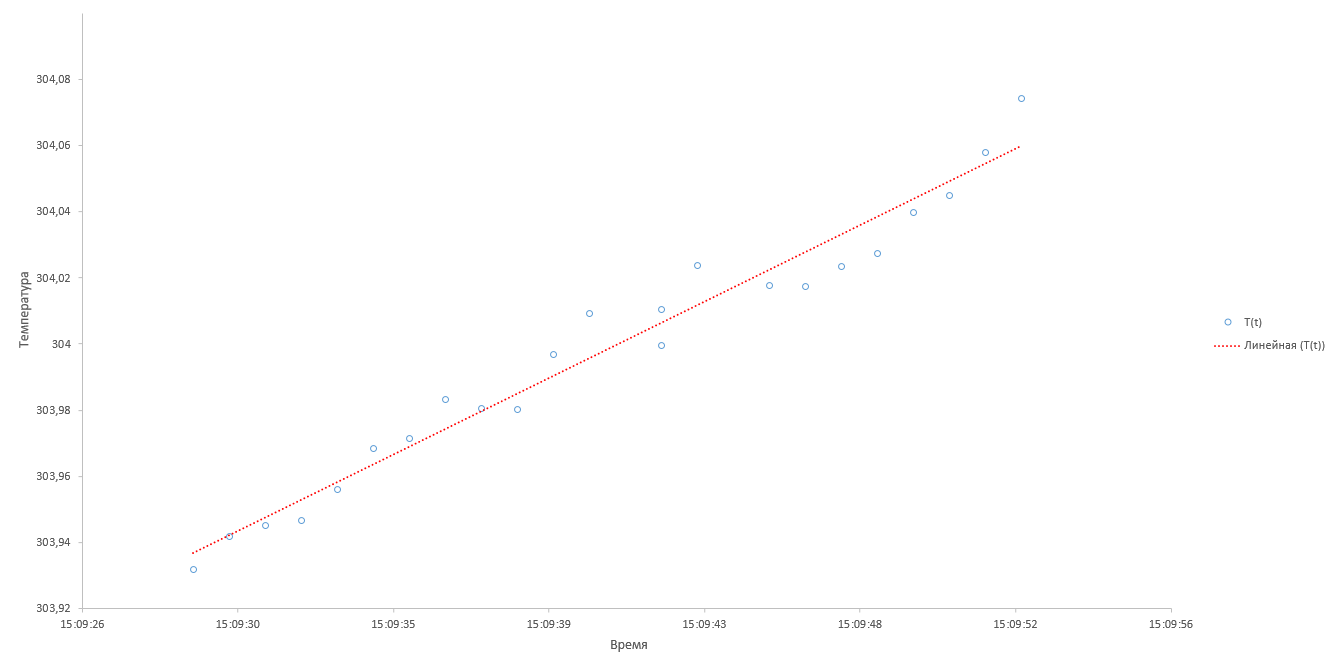
\includegraphics[width=1\linewidth]{картинки/2023-02-12_00-06-26.png}
				\caption{Пустой калориметр 1} %% подпись к рисунку
				\label{ris:dR_dt(r)_for_calorimetr} %% метка рисунка для ссылки на него
			\end{minipage}
		\hfill
			\begin{minipage}[h]{0.48\linewidth}
				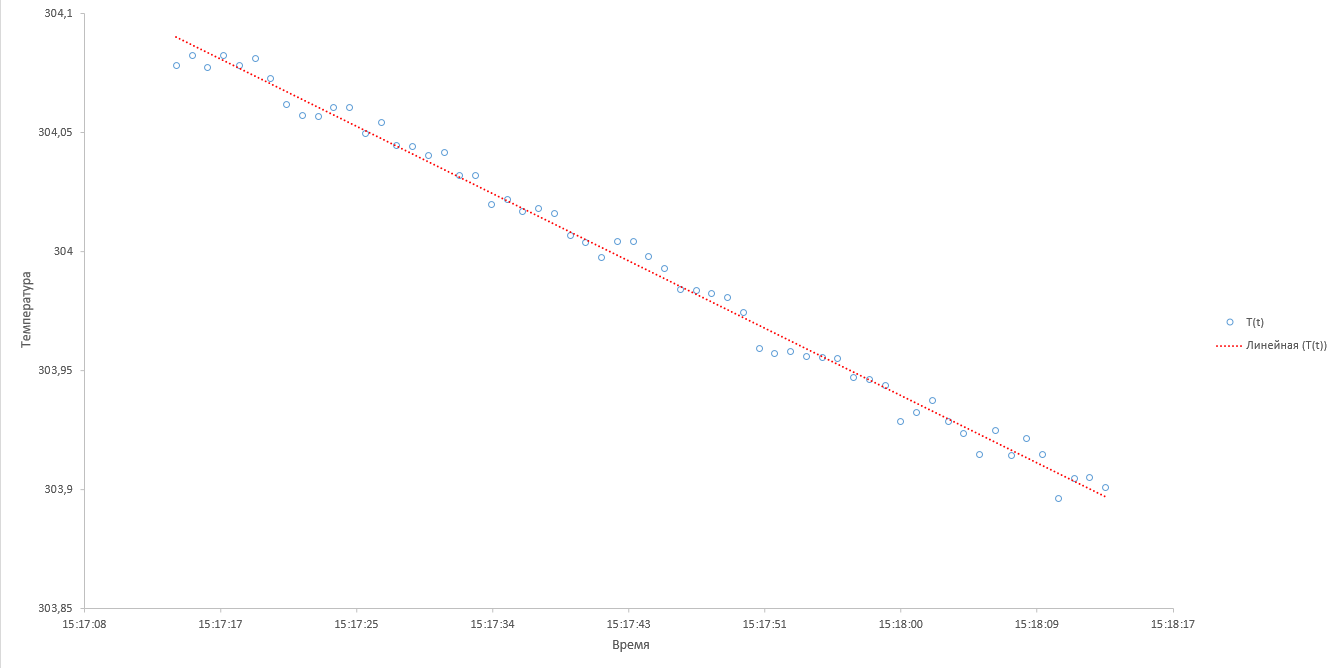
\includegraphics[width=1\linewidth]{картинки/2023-02-12_00-07-16.png}
				\label{ris:dR_dt(r)_for_steel}
			\end{minipage}
		\end{center}
		\begin{center}
			\begin{minipage}[h]{0.48\linewidth}
				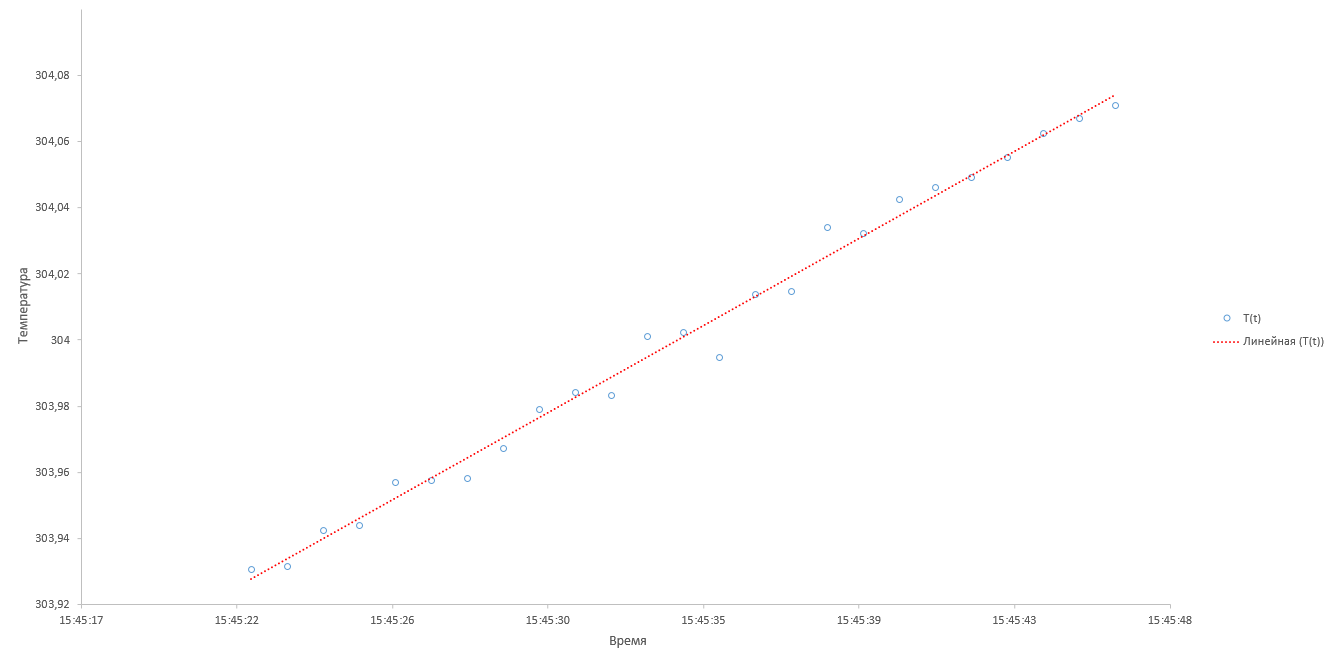
\includegraphics[width=1\linewidth]{картинки/2023-02-12_00-08-06.png}
				\caption{Пустой калориметр 2} 
				\label{ris:dR_dt(r)_for_latun'} %% метка рисунка для ссылки на него
			\end{minipage}
		\hfill
			\begin{minipage}[h]{0.48\linewidth}
				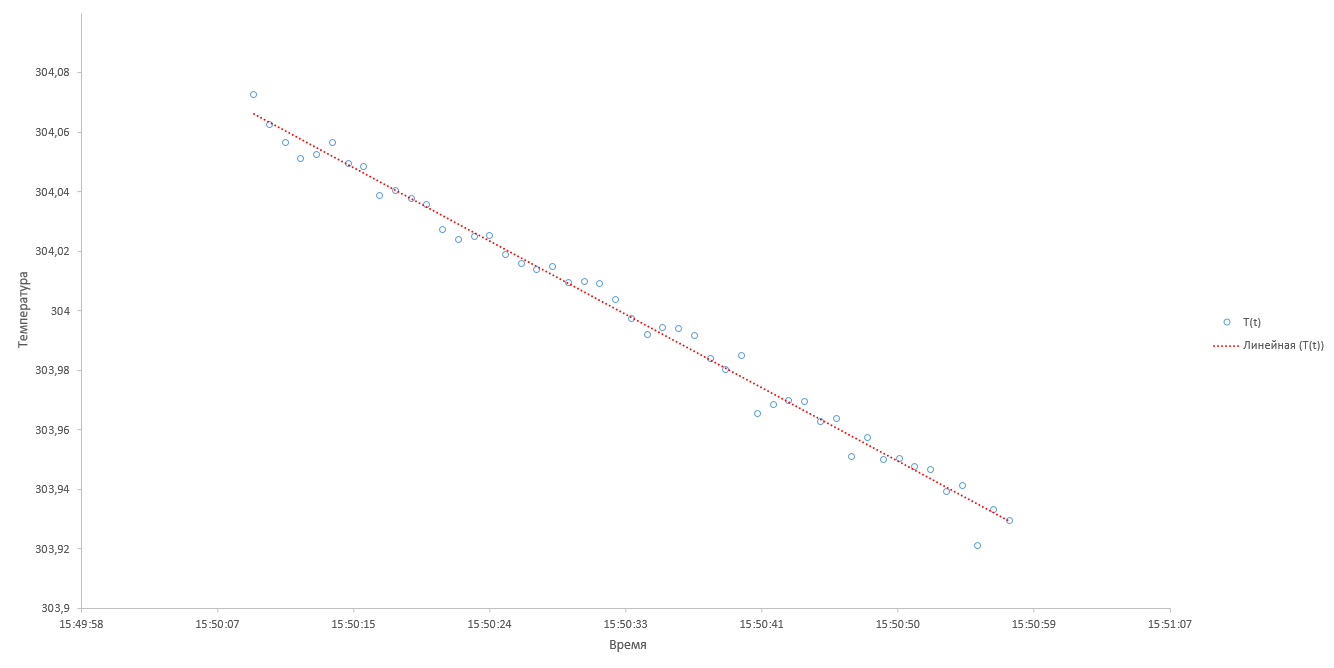
\includegraphics[width=1\linewidth]{картинки/2023-02-12_00-08-58.png}
				\label{ris:dR_dt(r)_for_aluminium}
			\end{minipage}
		\end{center}
				\begin{center}
			\begin{minipage}[h]{0.48\linewidth}
				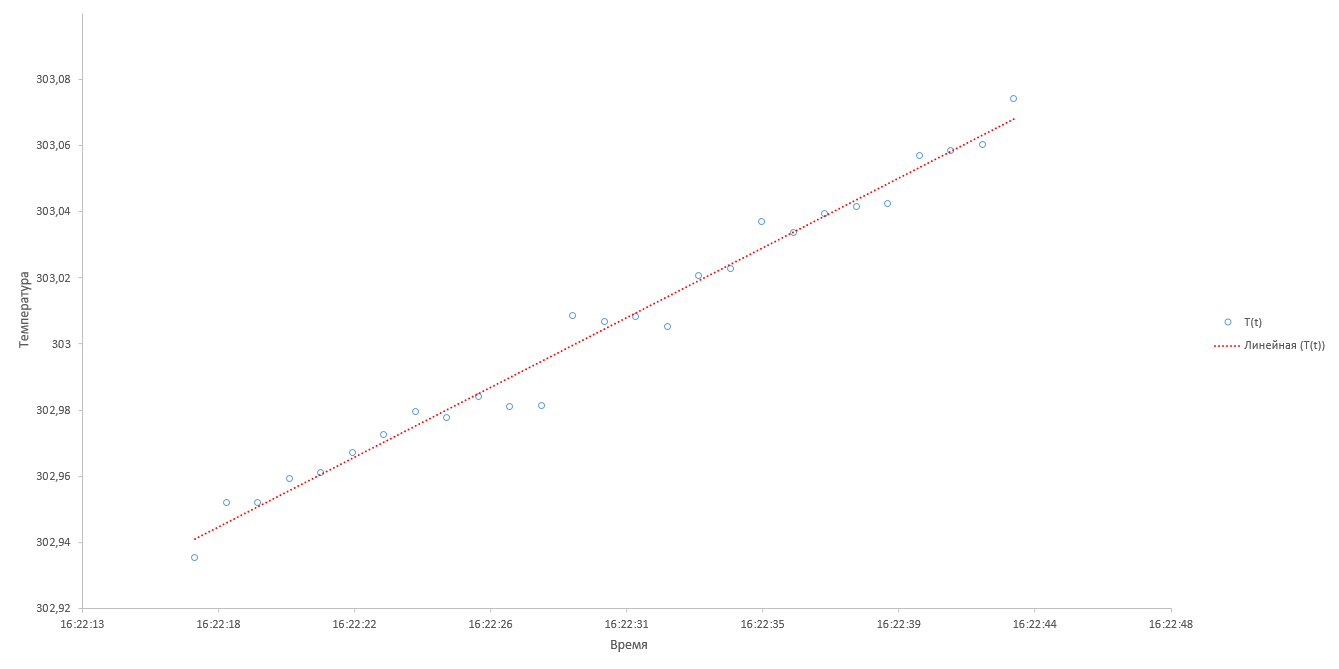
\includegraphics[width=1\linewidth]{картинки/2023-02-12_00-09-57.png}
				\caption{Алюминий} 
				\label{ris:dR_dt(r)_for_latun'} %% метка рисунка для ссылки на него
			\end{minipage}
		\hfill
			\begin{minipage}[h]{0.48\linewidth}
				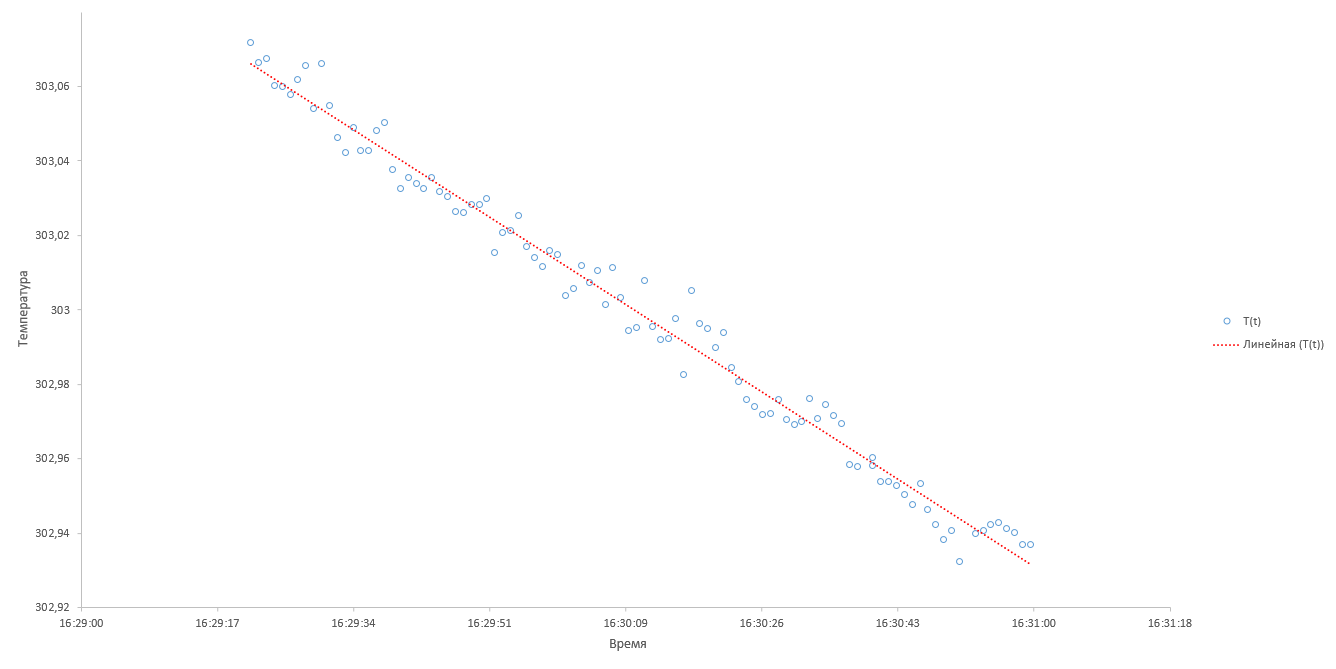
\includegraphics[width=1\linewidth]{картинки/2023-02-12_00-10-48.png}
				\label{ris:dR_dt(r)_for_aluminium}
			\end{minipage}
		\end{center}
\end{figure}

\newpage

Найду с помощью МНК коэффициенты A и B наклона графиков

\begin{center}
\begin{tabular}{|c|c|c|c|c|}
\hline
& A & B & $T_{k1}$, K & $T_{k2}$, K  \\
\hline
Пустой 1 & $(0.00569 \pm 0.00021)$ & $(-0.003272 \pm 0.000038)$ & 297.49 & 297.61 \\

Пустой 2 & $(0.00610 \pm 0.00013)$ & $(-0.002852 \pm 0.000042)$ & 298.08 & 298.13 \\	

Алюминий & $(0.00488 \pm 0.00013)$ & $(-0.001366 \pm 0.000018)$ & 298.45 & 298.53 \\
\hline
\end{tabular}
\end{center}

А также среднюю комнатную температуру на момент замера

Рассчитаю по теоретическим формулам теплоемкость и коэффициент теплопроводности

\begin{center}
\begin{tabular}{|c|c|c|}
\hline
& $\lambda$, $\frac{\text{Вт}}{K}$ & C, $\frac{\text{Дж}}{K}$ \\
\hline
Пустой 1 & $(0.350 \pm 0.016)$ & $(690 \pm 20)$ \\

Пустой 2 & $(0.334 \pm 0.009)$ & $(691 \pm 13)$ \\	

Алюминий & $(0.300 \pm 0.010)$ & $(990 \pm 20)$ \\
\hline
\end{tabular}
\end{center}

\subsection{Сведение в таблицу}

Ниже сведу все полученные данные в единую таблицу и произведу усреднение из расчета указанных погрешностей величин

\begin{center}
\begin{tabular}{|r|l|l|l|}
\hline
& Интегральный & Дифференциальный & II Дифференциальный \\
\hline
Калориметр 1; C, $\frac{\text{Дж}}{K}$ & $(697 \pm 3)$ & $(740 \pm 20)$ & $(690 \pm 20)$ \\
$\lambda$, $\frac{\text{Вт}}{K}$ & $(0.3598 \pm 0.0006)$ & & $(0.350 \pm 0.016)$ \\
Калориметр 2; C, $\frac{\text{Дж}}{K}$ & $(667 \pm 3)$ & $(670 \pm 30)$ & $(691 \pm 13)$ \\
$\lambda$, $\frac{\text{Вт}}{K}$ & $(0.3354 \pm 0.0003)$ & & $(0.334 \pm 0.009)$ \\
Калориметр ср.; C, $\frac{\text{Дж}}{K}$ & $(682 \pm 3)$ & $(710 \pm 30)$ & $(691 \pm 17)$ \\
$\lambda$, $\frac{\text{Вт}}{K}$ & $(0.3476 \pm 0.0005)$ & & $(0.342 \pm 0.0013)$ \\
\hline
Cal+Алюминий; C, $\frac{\text{Дж}}{K}$ & $(951 \pm 3)$ & $(970 \pm 40)$ & $(990 \pm 20)$ \\
$\lambda$, $\frac{\text{Вт}}{K}$ & $(0.2788 \pm 0.0003)$ & & $(0.300 \pm 0.010)$ \\
Алюминий; C, $\frac{\text{Дж}}{K}$ & $(269 \pm 6)$ & $(260 \pm 70)$ & $(300 \pm 40)$ \\
\hline
Cal + Железо; C, $\frac{\text{Дж}}{K}$ & & $(970 \pm 20)$ & \\
Железо; C, $\frac{\text{Дж}}{K}$ & & $(260 \pm 50)$ & \\
\hline
\end{tabular}
\end{center}

Усредню результаты всех методик, среднее значение вычислю средним арифметическим величин, предполагая равную достоверность всех экспериментов.

Погрешность вычислю таким образом

\begin{equation}
	\sigma_x = \sqrt{\sigma_{\text{стат}}^2 + \text{СР.АР}(\text{ПОГР}_i)^2}
\end{equation}

И пересчитаю темлоемкости металлов в удельные, пользуясь таблицей масс

\begin{center}
\begin{tabular}{|l|c|c|c|}
\hline
& C, $\frac{\text{Дж}}{K}$ & с, $\frac{\text{Дж}}{\text{кг} \cdot K}$ & $\lambda$, $\frac{\text{Вт}}{K}$ \\
\hline
Калориметр & $(694 \pm 19)$ & - & $(0.345 \pm 0.004)$ \\
\hline
Алюминий & $(280 \pm 40)$ & $(950 \pm 140)$ & $(0.289 \pm 0.011)$ \\
\hline
Железо & $(260 \pm 50)$ & $(320 \pm 60)$ & - \\
\hline
\end{tabular}
\end{center}

Дифференциальные методы сопряжены с большой погрешностью, приведу также таблицу, получаемую только интегральным методом.

\begin{center}
\begin{tabular}{|l|c|c|c|}
\hline
& C, $\frac{\text{Дж}}{K}$ & с, $\frac{\text{Дж}}{\text{кг} \cdot K}$ & $\lambda$, $\frac{\text{Вт}}{K}$ \\
\hline
Калориметр & $(682 \pm 3)$ & - & $(0.3476 \pm 0.0005)$ \\
\hline
Алюминий & $(269 \pm 6)$ & $(910 \pm 20)$ & $(0.2788 \pm 0.0003)$ \\
\hline
\end{tabular}
\end{center}

\section{Вывод}

В процессе работы было исследовано 2 дифференциальных и 1 интегральный метод. В результате были получены всевозможные значения теплоемкостей и коэффициента теплоотдачи стенок. По вычисленным значениям можно сказать, что интегральный метод значительно точнее дифференциальных при малых колебаниях комнатной температуры. При больших колебаниях передача тепла будет происходить нестационарно, и все методы могут давать значительно отличные от реальности результаты.

Удельная теплоемкость алюминия близка к табличному значению. Для железа она отличается довольно сильно. Могу предположить, что поскольку железо замерялось дифференциальным методом, и в самом конце работы, при пересечении комнатной температуры не успело установиться равновесное состояние. Это объясняет заниженность значения.

Поскольку было проведено прямое измерение кривых нагревания и охлаждения калориметра с телами внутри, определен коэффициент теплоотдачи стенок и теплоемкости калориметра и металлов конусов, буду считать цель работы выполненной.

\section{Ресурсы}

Расчет по МНК: метод-наименьших-квадратов.рф


\end{problem}
\end{document}